\section{Introduction}

The Salomon Islands are located in the central Indian Ocean (~5\degree 19'0'' S, 72\degree 15'36'' E) approximately 320 nautical miles south of the equator (Figure \ref{Chagos_fig1}). They collectively delimit the borders of one of the atolls of the Chagos Archipelago and provide shelter to the few yachts crossing the Indian Ocean, which, if granted a permit, may anchor in the pristine waters of the lagoon. After the forced relocation of the native Chagossian people, Chagos Archipelago has remained uninhabited except for British and American military personnel located on Diego Garcia, more than 100 nautical miles south of Salomon. The Chagos Archipelago has now become the British Indian Ocean Territory (BIOT), which comprises seven atolls and over 1000 islands spread over approximately 640,000 square kilometers. BIOT was established as a marine protected area in 2010, banning extraction activity and doubling the size of the no-take zones worldwide.\cite{sheppard2012reefs}

\begin{figure}
    \centering
    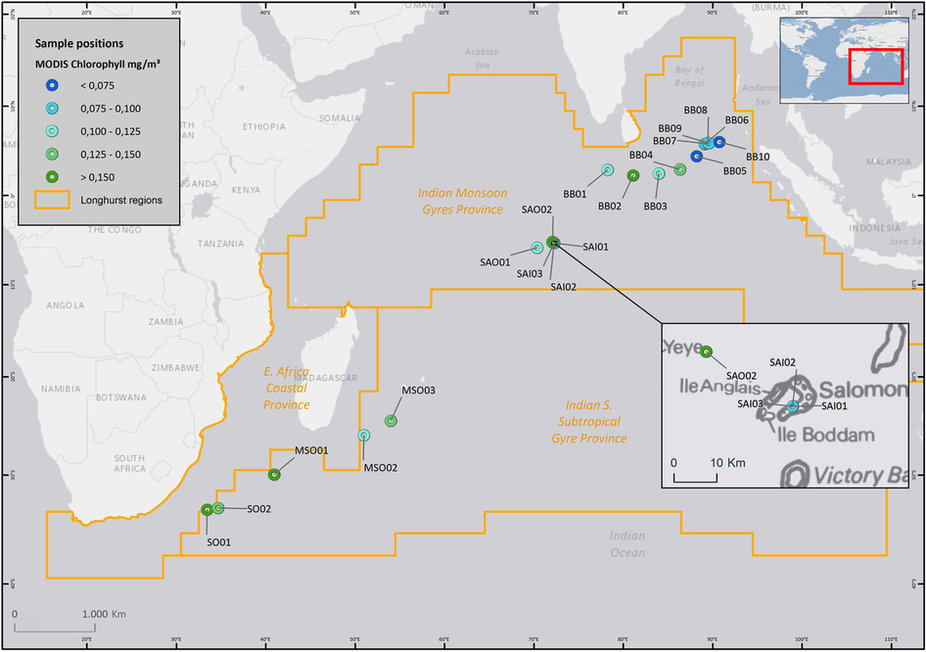
\includegraphics[width=\textwidth]{Chagos/figures/fig1}
    \caption{\textbf{Location of the samples in relation to the Longhurst provinces of the Indian Ocean.} \cite{rosenberg_role_2007} The chlorophyll concentration of each sample was estimated from MODIS data using ESRI's ArcGIS 10.3 Desktop as described in the methods.}
    \label{Chagos_fig1}
\end{figure}

ull size image
As a result of the limited anthropogenic input, its remote location and the proximity to the equator which shelters it from tropical cyclones, it has flourished as one of the healthiest coral reefs and has some of the cleanest waters in the world. \cite{sheppard2012reefs, riegl_human_2012}

While the Indian Ocean is generally considered oligotrophic, the enhanced productivity around the Chagos Archipelago \cite{sheppard1999ecology} is a result of the combined effects of Ekman pumping \cite{sheppard2012reefs, resplandy2009seasonal} and ocean currents hitting the Chagos seamounts. \cite{sheppard1999ecology, mendonca_is_2012}

While conservation efforts have been in place to maintain the integrity of the macro-faunal portion of the reef ecosystem, much less is known about the microbial community. Coral reefs, like most other ecosystems are intrinsically dependent on healthy microbial communities. \cite{dinsdale_microbial_2008, rosenberg_role_2007}

Because of their abundance and functional role, microbes are the key providers of ecosystem services, acting as early sentinels of environmental change. Monitoring the marine microbiome is a useful parameter that can be used to detect changes and potential deleterious effects in any given ecosystem. Such information could be useful in efforts to better manage and protect fisheries, ecosystems and the greater ocean basin.

However, few studies have attempted to characterise the marine microbiome's resilience and response to environmental perturbations, which as a first step, requires the establishment of baselines for diversity, functional capacity and activity of the autochthonous microbiome.

Here for the first time, the genetic diversity and transcriptional dynamics of the microbial community in the lagoon of the Salomon Islands is described. This dataset provides an insight into the unique microbiota of the lagoon, spanning viruses, bacteria and microbial eukaryotes and provides a baseline for future monitoring activities and conservation efforts. Moreover, this study was entirely conducted using a private sailboat serving as a proof of concept that `citizen oceanographers' can contribute to our scientific perspective in a rigorous and meaningful way. \cite{lauro_common_2014}